\newpage
\chapter{Hardware implementation}
\label{sec:implementation}
\section{Memory management}
\label{sec:memory_management}
\subsection{Correlation matrix}
\label{sec:mem_management_correlation_matrix}
Storing and updating the causal correlation matrix sum as shown in equation \ref{eq:caus_corr} requires a lot of memory resources. This update needs to be done for each pixel in the image, and the memory used for this operation is therefore important in order to make the AD real-time. The size of the correlation matrix will be $p * p$, where $p$ is the number of spectral bands in the image. As mentioned, the number of usable bands $N_{bands}$ is 100. The image pixel data width, $pixel\_data\_width$ is assumed to be 16 bit/band/pixel. As the correlation matrix is the product of $\textbf{x}$ * $\textbf{x}^T$ the resulting width will be 2* $pixel\_data\_width$. Using spectral information from all the bands would require $p * p * 32$= $100$ *$100$ *$32$ bit = $320 kbit$ of memory storage. 
\\

There are three alternatives to storing all this information on the FPGA, storing it in block RAM, distributed RAM or in registers. The FPGA to be used in the SmallSat's first prototype is the Zynq Z-7030 or Zynq Z-7035. It contains the memory resources as shown in figure \ref{fig:zynq_memory_resources}.





\begin{figure}[H]
\centering                                                           

   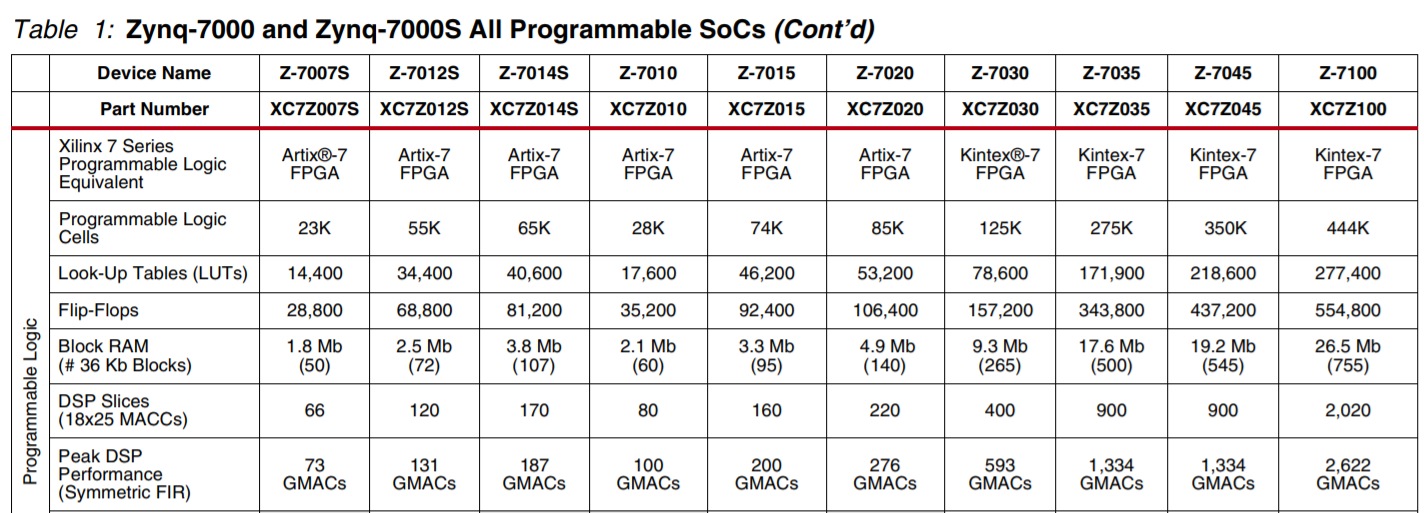
\includegraphics[scale=0.5]{images/zynq_memory_resources.PNG}
  \caption{Zynq memory resources, found in \cite{cite:mem_resources_zynq}} 
  \label{fig:zynq_memory_resources}.
\end{figure}

\subsubsection{Using registers}
The Zynq Z-7030 and the Zynq Z-7035 have $157,200$ and $343,800$ flip flops each, respectively. Using equation \ref{eq:max_bands}, the maximal number of spectral bands used is 70 and 103. However, this is unrealistic as this leaves no free flip flop free in the design. As the AD implemented in this task is a part of a larger processing pipeline (insert picture of pipeline somewhere?) it is not acceptable to use all of the available flip flops. Assuming that it is acceptable to use 15\% of the available flip flops, the number of spectral bands that can be used is 27 and 40. This dimensional reduction can be done through pre-prossesing of data by for example Principal Component Analysis(PCA). (insert result showing AD doing better with PCA in front?). 
The benefit of the use of registers is the speed and the ability of instantaneous update (after a clock cycle). This will lead to the AD becoming closer to real-time than if distributed RAM or BRAM is used.

\begin{equation}
    max\_bands= \sqrt{\frac{number\_of\_registers}{2*pixel\_data\_width}}
    \label{eq:max_bands}
\end{equation}

\subsubsection{Using BRAM}
The Z-7030 and the Z-7035 contains 265 and 500 $36$kbit BRAM - blocks. In  order to store the largest correlation matrix of $320 kbit$ 9 BRAM blocks are needed. Each 36 kbit BRAM block consists of two 18 kbit BRAM blocks. In true dual port(TDP) mode \cite{cite:ug953}, it is possible to do two writes and two reads per BRAM each clock cycle, with each write and read being maximum 36 bits. Equation \ref{eq:clk_cycles_corr_update_BRAM} shows the calculation of number of clock cycles needed to update the correlation matrix, $n\_clk\_update\_corr\_BRAM$. This is done for each pixel in the image. $n\_BRAM$ is the number of BRAM used to store the correlation matrix. The total time spent updating the correlation matrix for the entire image is given by equation \ref{eq:clk_cycles_corr_image}. Updating a correlation matrix wih $p$ = 100, using 9 BRAMs in TDP mode would require 556 clk cycles. For the entire image, having $N\_pixels$ the total amount of clock cycles spent updating the correlation matrix would be 349648384. At a target clock frequency of 100 MHz this would require $3.49648$ seconds, which is not to be considered real time.   

\begin{equation}
    n\_clk\_update\_corr\_BRAM = \frac{p * p }{2 * n\_BRAM}
    \label{eq:clk_cycles_corr_update_BRAM}
\end{equation}

\begin{equation}
    clk\_corr\_image\_BRAM = N\_pixels *number\_of\_lines * n\_clk\_update\_corr\_BRAM
    \label{eq:clk_cycles_corr_image}
\end{equation}


Figure \ref{fig:update_time_correlation_BRAM} shows the total time spent updating the correlation matrix for a image of 1088 pixel rows with 578 effective pixels per row, with a target clock frequency of 100 MHz. The BRAMs are assumed written to in parallell.  

\begin{figure}[H]
\centering
   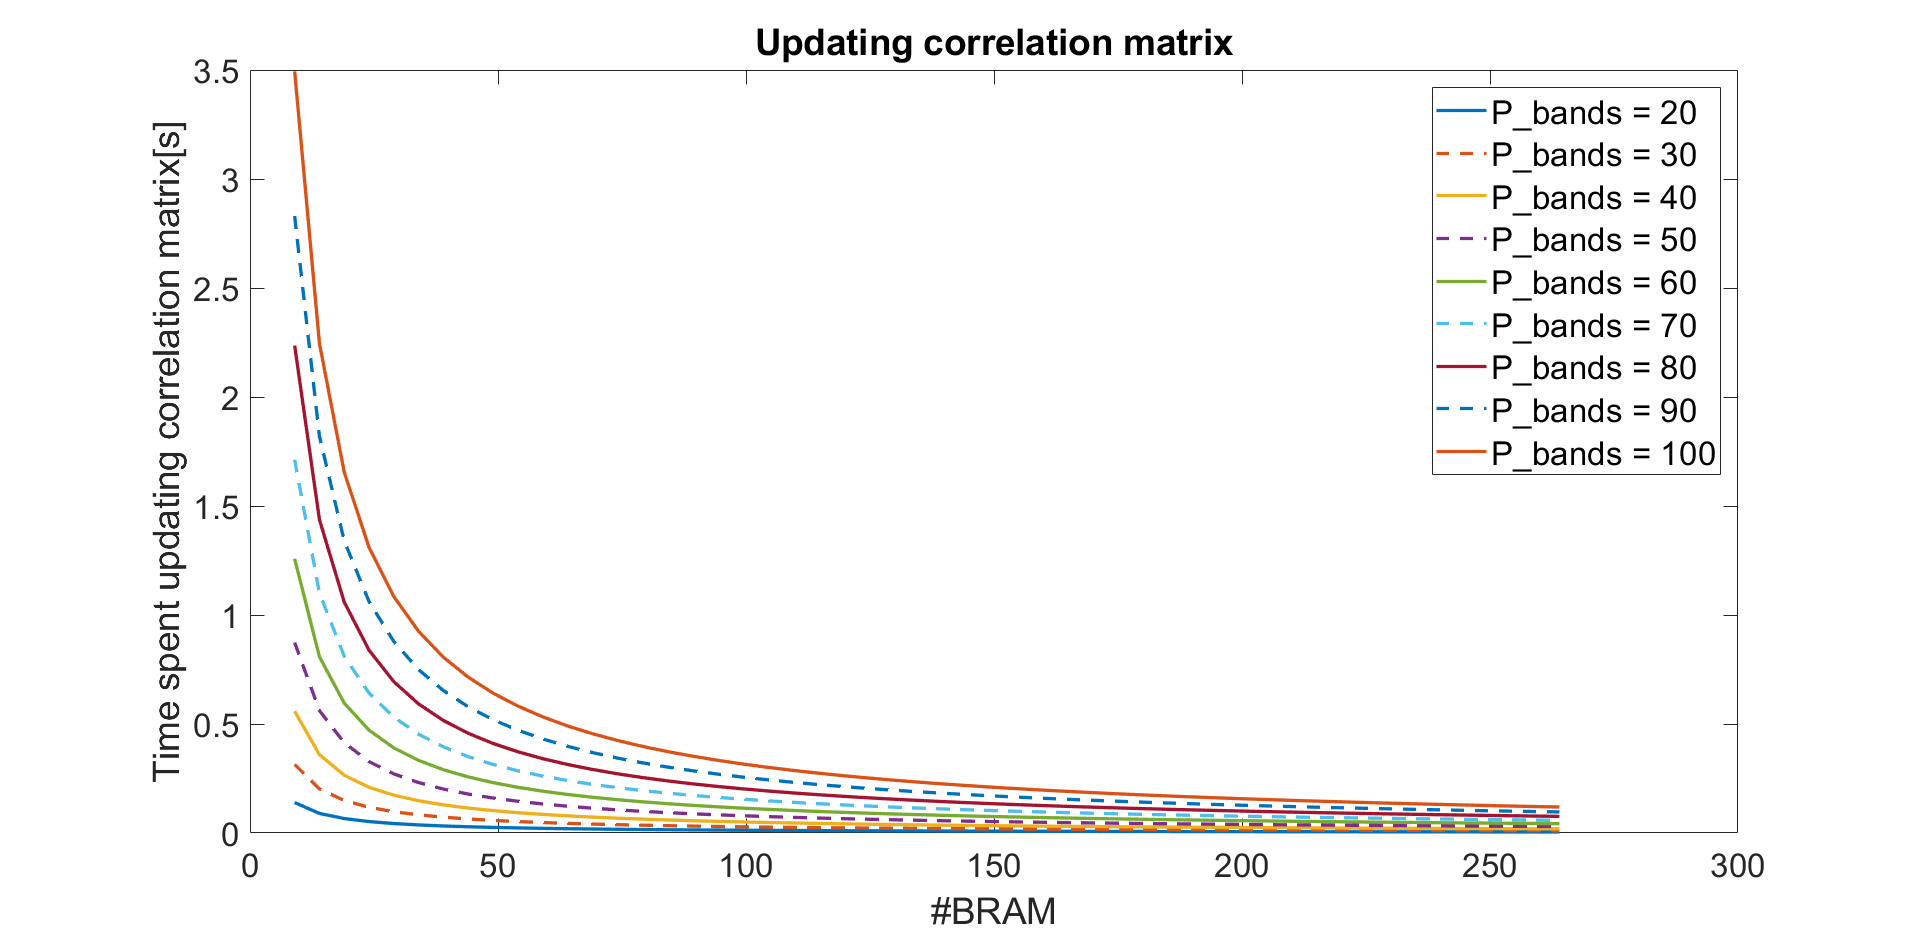
\includegraphics[scale=0.3]{images/time_spent_updating_correlation_matrix.png}
  \caption{Estimated time spent updating correlation matrix for an image of 1088 pixel rows with 578 effective pixel per row, with a target clock frequency of 100 MHz, plotted as a function of number of BRAMs used to store and update the correlation matrix. Plotted for spectral bands in the range of P=20 to P=100. } 
  \label{fig:update_time_correlation_BRAM}
\end{figure}

\section{ACAD correlation}
\label{sec:correlation_hw}
\subsection{Memory management}
As the design is in the early phases, the value of $p$ used throughout the project is insecure. Another insecurity is the performance of the ACAD AD using PCA pre-processing, i.e. reducing the number of spectral bands in the AD. In addition, the ACAD AD requires storing of the inverse matrix, and the sum of anomaly detected. This is shown in figure X ( insert a figure showing the equation and what needs to be stored where). It is therefore not desirable to store the entire correlation matrix in registers, as there will be a need for storing other matrices in BRAM or slower storage, thereby inserting a bottleneck in the pipeline.
\\

As shown in Figure \ref{fig:update_time_correlation_BRAM} the time spent updating the correlation matrix can be reduced by increasing number of BRAMs used to store the correlation matrix. By setting the  number of BRAMs used to store the correlation matrix, $N\_BRAMS\_correlation$, equal to $P\_BANDS$ the control logic is simplified while achieving an acceptable trade off between speedup as a function of number of BRAMs used and resources used. Figure \ref{fig:data_flow_cube_dma_to_inverse} shows the data flow from the Cube DMA through the ACAD correlation module. 


\begin{figure}[H]
\centering
   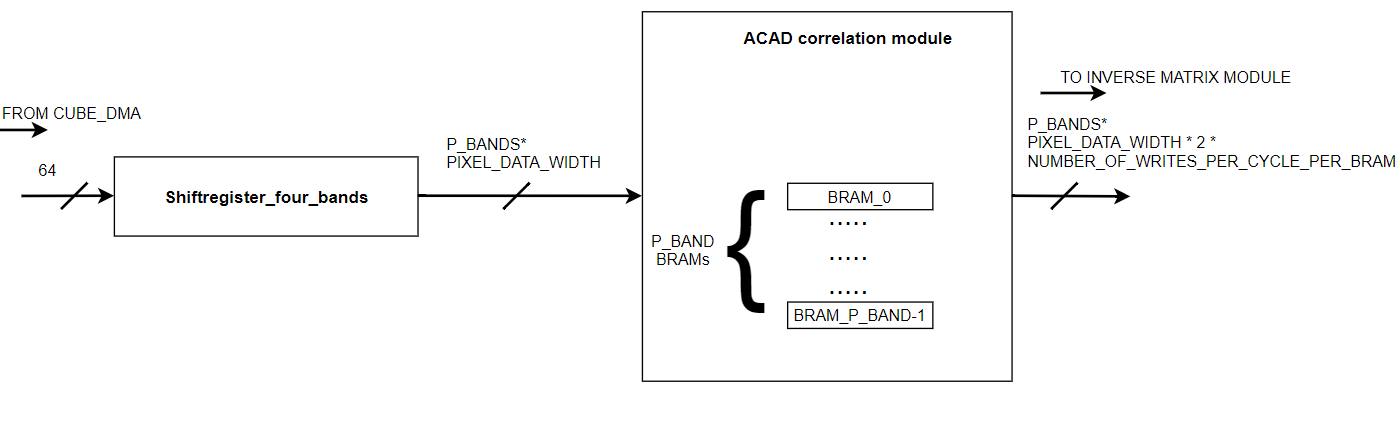
\includegraphics[scale=0.5]{images/data_flow_cube_dma_to_inverse_module.PNG}
  \caption{Data flow from Cube DMA via shiftregister to correlation module. Output on right hand side are input for inverse matrix computation module.  } 
  \label{fig:data_flow_cube_dma_to_inverse}
\end{figure}


\section{Inverse computation}
\label{sec:inverse_computation_hw}